%!TEX root = ../../msc17-game-book.tex


\phChapterWorksheet{Count on It}{Main Puzzle 4}

Count Calcula is planning construction for a new town called
``Batty Bourough'' outside Transylvania. As
everyone knows, the cost to construct a building is
\textbf{100 dragon teeth} per
road leading into that building. ``Ack! Vat a pain in the neck!
I vish someone vould help me by \textit{biting}, er, writing down
the cost of my building plan!''

\begin{center}
\begin{tikzpicture}[x=0.3in,y=0.2in]

  \coordinate (A) at (0,0);
  \node at (A) {\textbullet};
  \node[below=8] at (A) {Calcula's House};

  \coordinate (B) at (4,-4);
  \node at (B) {\textbullet};
  \node[below] at (B) {Starbucks};
      \coordinate (AB) at (3,-2);

  \coordinate (C) at (8,2);
  \node at (C) {\textbullet};
  \node[right] at (C) {Scaring School};
      \coordinate (BC) at (7,-2);

  \coordinate (D) at (6,6);
  \node at (D) {\textbullet};
  \node[above right] at (D) {Gargoyles Galore};
      \coordinate (AD) at (4,3);
      \coordinate (CD) at (7.5,4);

  \coordinate (E) at (3,5);
  \node at (E) {\textbullet};
  \node[above=4] at (E) {Monsters, LLC};
      \coordinate (DE) at (4,4.8);

  \coordinate (F) at (1,8);
  \node at (F) {\textbullet};
  \node[above right] at (F) {Capes \reflectbox{R} Us};
      \coordinate (EF) at (2,5);

  \coordinate (F') at (-1,8);
  \node at (F') {\textbullet};
  \node[above left] at (F') {Rat Hats};
      \coordinate (FF') at (0,7.5);

  \coordinate (E') at (-3,5);
  \node at (E') {\textbullet};
  \node[above=4] at (E') {Sun Blocker};
      \coordinate (E'F') at (-2,5);

  \coordinate (D') at (-6,6);
  \node at (D') {\textbullet};
  \node[above=4] at (D') {Blood Bank};
      \coordinate (AD') at (-4,3);
      \coordinate (D'E') at (-4,4.8);

  \coordinate (C') at (-8,2);
  \node at (C') {\textbullet};
  \node[left] at (C') {Werewolf Puck's};
      \coordinate (C'D') at (-7.5,4);

  \coordinate (B') at (-4,-4);
  \node at (B') {\textbullet};
  \node[below] at (B') {Cozy Coffins};
      \coordinate (B'C') at (-7,-2);
      \coordinate (AB') at (-3,-2);

  \draw (A)
        to[arc through cw={(AB)}] (B);
  \draw (A) -- (C);
  \draw (A)
        to[arc through ccw={(AD)}] (D);
  \draw (A) -- (E);
  \draw (A) -- (E');
  \draw (A)
        to[arc through cw={(AD')}] (D');
  \draw (A) -- (C');
  \draw (A)
      to[arc through ccw={(AB')}] (B');
  \draw (B)
        to[arc through ccw={(BC)}] (C);
  \draw (C)
        to[arc through ccw={(CD)}] (D);
  \draw (D)
        to[arc through cw={(DE)}] (E);
  \draw (E)
        to[arc through cw={(EF)}] (F);
  \draw (F)
        to[arc through cw={(FF')}] (F');
  \draw (E')
        to[arc through ccw={(E'F')}] (F');
  \draw (D')
        to[arc through ccw={(D'E')}] (E');
  \draw (C')
        to[arc through cw={(C'D')}] (D');
  \draw (B')
        to[arc through cw={(B'C')}] (C');
\end{tikzpicture}
\end{center}

\noindent\textbf{What would be the total cost of building Batty Bourough?}

% 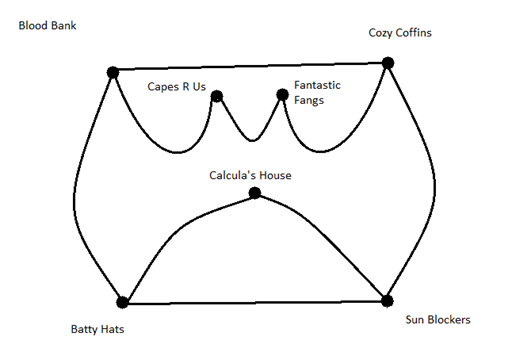
\includegraphics[scale=.7]{assets/josh/planb}

\vspace{3em}

Actually, the Count's ulimate goal is to renovate all of Transylvania itself,
a monsterous metropolis with \textbf{57 buildings} and \textbf{73 roads}.
He calculates that renovating each building would only cost
\textbf{50 dragon teeth}
per road leading into it, but he cannot seem to track down a roadmap
similar to his plan for Batty Borough. All he knows is that each road
begins and ends at a building.
\textbf{Does the
Count have enough information to calculuate the cost of renovating
Transylvania? If so, what would the renovation cost?}
